\documentclass[]{book}
\usepackage{lmodern}
\usepackage{amssymb,amsmath}
\usepackage{ifxetex,ifluatex}
\usepackage{fixltx2e} % provides \textsubscript
\ifnum 0\ifxetex 1\fi\ifluatex 1\fi=0 % if pdftex
  \usepackage[T1]{fontenc}
  \usepackage[utf8]{inputenc}
\else % if luatex or xelatex
  \ifxetex
    \usepackage{mathspec}
  \else
    \usepackage{fontspec}
  \fi
  \defaultfontfeatures{Ligatures=TeX,Scale=MatchLowercase}
\fi
% use upquote if available, for straight quotes in verbatim environments
\IfFileExists{upquote.sty}{\usepackage{upquote}}{}
% use microtype if available
\IfFileExists{microtype.sty}{%
\usepackage{microtype}
\UseMicrotypeSet[protrusion]{basicmath} % disable protrusion for tt fonts
}{}
\usepackage[margin=1in]{geometry}
\usepackage{hyperref}
\hypersetup{unicode=true,
            pdftitle={Teaching and Learning with Jupyter},
            pdfauthor={Lorena A. Barba et al.},
            pdfborder={0 0 0},
            breaklinks=true}
\urlstyle{same}  % don't use monospace font for urls
\usepackage{natbib}
\bibliographystyle{apalike}
\usepackage{color}
\usepackage{fancyvrb}
\newcommand{\VerbBar}{|}
\newcommand{\VERB}{\Verb[commandchars=\\\{\}]}
\DefineVerbatimEnvironment{Highlighting}{Verbatim}{commandchars=\\\{\}}
% Add ',fontsize=\small' for more characters per line
\usepackage{framed}
\definecolor{shadecolor}{RGB}{248,248,248}
\newenvironment{Shaded}{\begin{snugshade}}{\end{snugshade}}
\newcommand{\KeywordTok}[1]{\textcolor[rgb]{0.13,0.29,0.53}{\textbf{#1}}}
\newcommand{\DataTypeTok}[1]{\textcolor[rgb]{0.13,0.29,0.53}{#1}}
\newcommand{\DecValTok}[1]{\textcolor[rgb]{0.00,0.00,0.81}{#1}}
\newcommand{\BaseNTok}[1]{\textcolor[rgb]{0.00,0.00,0.81}{#1}}
\newcommand{\FloatTok}[1]{\textcolor[rgb]{0.00,0.00,0.81}{#1}}
\newcommand{\ConstantTok}[1]{\textcolor[rgb]{0.00,0.00,0.00}{#1}}
\newcommand{\CharTok}[1]{\textcolor[rgb]{0.31,0.60,0.02}{#1}}
\newcommand{\SpecialCharTok}[1]{\textcolor[rgb]{0.00,0.00,0.00}{#1}}
\newcommand{\StringTok}[1]{\textcolor[rgb]{0.31,0.60,0.02}{#1}}
\newcommand{\VerbatimStringTok}[1]{\textcolor[rgb]{0.31,0.60,0.02}{#1}}
\newcommand{\SpecialStringTok}[1]{\textcolor[rgb]{0.31,0.60,0.02}{#1}}
\newcommand{\ImportTok}[1]{#1}
\newcommand{\CommentTok}[1]{\textcolor[rgb]{0.56,0.35,0.01}{\textit{#1}}}
\newcommand{\DocumentationTok}[1]{\textcolor[rgb]{0.56,0.35,0.01}{\textbf{\textit{#1}}}}
\newcommand{\AnnotationTok}[1]{\textcolor[rgb]{0.56,0.35,0.01}{\textbf{\textit{#1}}}}
\newcommand{\CommentVarTok}[1]{\textcolor[rgb]{0.56,0.35,0.01}{\textbf{\textit{#1}}}}
\newcommand{\OtherTok}[1]{\textcolor[rgb]{0.56,0.35,0.01}{#1}}
\newcommand{\FunctionTok}[1]{\textcolor[rgb]{0.00,0.00,0.00}{#1}}
\newcommand{\VariableTok}[1]{\textcolor[rgb]{0.00,0.00,0.00}{#1}}
\newcommand{\ControlFlowTok}[1]{\textcolor[rgb]{0.13,0.29,0.53}{\textbf{#1}}}
\newcommand{\OperatorTok}[1]{\textcolor[rgb]{0.81,0.36,0.00}{\textbf{#1}}}
\newcommand{\BuiltInTok}[1]{#1}
\newcommand{\ExtensionTok}[1]{#1}
\newcommand{\PreprocessorTok}[1]{\textcolor[rgb]{0.56,0.35,0.01}{\textit{#1}}}
\newcommand{\AttributeTok}[1]{\textcolor[rgb]{0.77,0.63,0.00}{#1}}
\newcommand{\RegionMarkerTok}[1]{#1}
\newcommand{\InformationTok}[1]{\textcolor[rgb]{0.56,0.35,0.01}{\textbf{\textit{#1}}}}
\newcommand{\WarningTok}[1]{\textcolor[rgb]{0.56,0.35,0.01}{\textbf{\textit{#1}}}}
\newcommand{\AlertTok}[1]{\textcolor[rgb]{0.94,0.16,0.16}{#1}}
\newcommand{\ErrorTok}[1]{\textcolor[rgb]{0.64,0.00,0.00}{\textbf{#1}}}
\newcommand{\NormalTok}[1]{#1}
\usepackage{longtable,booktabs}
\usepackage{graphicx,grffile}
\makeatletter
\def\maxwidth{\ifdim\Gin@nat@width>\linewidth\linewidth\else\Gin@nat@width\fi}
\def\maxheight{\ifdim\Gin@nat@height>\textheight\textheight\else\Gin@nat@height\fi}
\makeatother
% Scale images if necessary, so that they will not overflow the page
% margins by default, and it is still possible to overwrite the defaults
% using explicit options in \includegraphics[width, height, ...]{}
\setkeys{Gin}{width=\maxwidth,height=\maxheight,keepaspectratio}
\IfFileExists{parskip.sty}{%
\usepackage{parskip}
}{% else
\setlength{\parindent}{0pt}
\setlength{\parskip}{6pt plus 2pt minus 1pt}
}
\setlength{\emergencystretch}{3em}  % prevent overfull lines
\providecommand{\tightlist}{%
  \setlength{\itemsep}{0pt}\setlength{\parskip}{0pt}}
\setcounter{secnumdepth}{5}
% Redefines (sub)paragraphs to behave more like sections
\ifx\paragraph\undefined\else
\let\oldparagraph\paragraph
\renewcommand{\paragraph}[1]{\oldparagraph{#1}\mbox{}}
\fi
\ifx\subparagraph\undefined\else
\let\oldsubparagraph\subparagraph
\renewcommand{\subparagraph}[1]{\oldsubparagraph{#1}\mbox{}}
\fi

%%% Use protect on footnotes to avoid problems with footnotes in titles
\let\rmarkdownfootnote\footnote%
\def\footnote{\protect\rmarkdownfootnote}

%%% Change title format to be more compact
\usepackage{titling}

% Create subtitle command for use in maketitle
\newcommand{\subtitle}[1]{
  \posttitle{
    \begin{center}\large#1\end{center}
    }
}

\setlength{\droptitle}{-2em}

  \title{Teaching and Learning with Jupyter}
    \pretitle{\vspace{\droptitle}\centering\huge}
  \posttitle{\par}
    \author{Lorena A. Barba et al.}
    \preauthor{\centering\large\emph}
  \postauthor{\par}
      \predate{\centering\large\emph}
  \postdate{\par}
    \date{2018-11-30}

\usepackage{booktabs}
\usepackage{amsthm}
\makeatletter
\def\thm@space@setup{%
  \thm@preskip=8pt plus 2pt minus 4pt
  \thm@postskip=\thm@preskip
}
\makeatother

\begin{document}
\maketitle

{
\setcounter{tocdepth}{1}
\tableofcontents
}
\chapter{Prerequisites}\label{prerequisites}

This is a \emph{sample} book written in \textbf{Markdown}. You can use
anything that Pandoc's Markdown supports, e.g., a math equation
\(a^2 + b^2 = c^2\).

The \textbf{bookdown} package can be installed from CRAN or Github:

\begin{Shaded}
\begin{Highlighting}[]
\KeywordTok{install.packages}\NormalTok{(}\StringTok{"bookdown"}\NormalTok{)}
\CommentTok{# or the development version}
\CommentTok{# devtools::install_github("rstudio/bookdown")}
\end{Highlighting}
\end{Shaded}

Remember each Rmd file contains one and only one chapter, and a chapter
is defined by the first-level heading \texttt{\#}.

To compile this example to PDF, you need XeLaTeX. You are recommended to
install TinyTeX (which includes XeLaTeX):
\url{https://yihui.name/tinytex/}.

\chapter{Introduction}\label{intro}

Project Jupyter is a broad collaboration that develops open-source tools
for interactive and exploratory computing. The tools include: IPython,
the Jupyter Notebook, Jupyter Hub, and an ecosystem of extensions
contributed by a large community. Jupyter Notebook exploded in
popularity since late 2014, fueled by its adoption as the favorite
environment for doing data science. It has also grown as a platform to
use in the classroom, to develop teaching materials, to share lessons
and tutorials, and more. Notebooks are documents containing text
narratives, combined with executable code (many languages are supported)
and the output of that code. This marriage of content and code makes for
a powerful new form of data-based communication. Educators everywhere
are adopting Jupyter for teaching.

This handbook is for any educator teaching a topic that includes data
analysis or computation to support the learning---not just courses in
engineering or science, but also data journalism, business and
quantitative economics, data-based decision sciences and policy,
quantitative health sciences, and others. It aims to give an entry
point, and a broad overview of Jupyter in education. Whether you are
already using Jupyter to teach, you have found learning materials built
on Jupyter that piqued your curiosity, or have never heard of Jupyter,
the material in this open book can help you empower your teaching with
this new technology.

Educators newly adopting Jupyter can be overwhelmed by having to
navigate the ecosystem of tools and content. They could study many
examples, or consume myriad blog posts and talk videos to distill the
patterns of good practices and technical solutions to best serve their
students. Several early adopters, having much experience to share,
decided to begin collecting this know-how, and sharing open
documentation about using Jupyter for teaching and learning.

The Jupyter Community Workshop in DC (November 2018) began that process,
with a book sprint aimed at producing the first version of this
handbook. The collaboratively written book consolidates explanations and
examples covering key topics, including: what is Jupyter, how to try
Jupyter, sharing notebooks with students, locally installing Jupyter,
cloud offerings, finding example notebooks, writing lessons in Jupyter,
making collections for a course, exporting to other formats with
nbconvert, writing textbooks with Jupyter, using Binder, JupyterHub,
making assignments and auto-grading, making online courses, teaching
with Jupyter in the classroom, active learning and flipped learning
pedagogies with Jupyter, guiding learners to create their own content in
Jupyter, and more. This open handbook will grow to encompass all you
need to know about Jupyter in Teaching and Learning.

If you find these materials helpful or inspiring, give us a shout-out on
Twitter using \#Jupyter4Edu. We hope you do!

\section{Acknowledgements}\label{acknowledgements}

The book sprint was held at the George Washington University in
Washington, DC, on 28--30 November 2018, and organized by Lorena A.
Barba. Funding to support the logistics and travel of all participants
was possible thanks to a grant from Bloomberg to Project Jupyter, and
managed by NumFOCUS. The group was fêted at a reception sponsored by
Leidos. Participants traveled from all over the country and volunteered
their precious time and hard work to give this work to the Jupyter
community, with a heartfelt sense of gratitude to all the contributors
to the software projects we love and depend on. Thank you!

GitHub repository for this book:
\url{https://github.com/jupyter4edu/jupyter-edu-book}

\chapter{Why we use Jupyter
Notebooks}\label{why-we-use-jupyter-notebooks}

\section{Introduction}\label{introduction}

In Chapter 2, you will be introduced to why and how educators are using
Jupyter Notebooks. We will highlight examples illustrating how notebooks
are being used to increase student engagement, participation,
understanding, and performance. Notebooks can also have benefits for
students that extend beyond your course, while also offering substantial
benefits to you, the teacher, over other tools.

\section{Why do we as educators use
Jupyter?}\label{why-do-we-as-educators-use-jupyter}

As teachers we are responsible for a vast array of activities, including
creating lessons, lectures, courses, assignments, and supportive
environments; encouraging engagement and performance in the classroom;
helping students learn to think critically so they can become lifelong
learners and problem solvers; making material relevant and meaningful to
students' diverse interests and backgrounds; assessing student learning
(including grading and evaluation); encouraging students to persist with
emotional labor (feedback, communication, etc.); and trying out teaching
and learning practices that improve our ability to do all of these
things.

In short, teachers design learning environments and experiences. We use
Jupyter Notebooks to design learning environments to help support these
activities. The goal of this handbook is to provide you with ideas to
help you address your own instructional and pedagogical goals. We
believe that incorporating Jupyter Notebooks in our teaching has allowed
us to help improve students' understanding of course content, help
increase student engagement and participation in class, and help make
concepts more meaningful and relevant to students' diverse interests. We
have found that this can be achieved in a variety disciplines and across
many diverse types of instructional goals.

Through a series of anecdotes we will illustrate how you, as an
educator, can help increase your students' 1) engagement, 2)
participation, 3) understanding, 4) performance, 5) preparation for
their career, using Jupyter notebooks. These are starting places and we
are confident that you will also take these examples in new and exciting
directions.

\section{But first, what is a Jupyter
Notebook?}\label{but-first-what-is-a-jupyter-notebook}

Project Jupyter is actually three things: a collection of standards, a
community, and a set of software tools. A Jupyter Notebook is one part
of Jupyter; it is a document that supports mixing executable code,
equations, visualizations, and narrative text. Specifically, Jupyter
Notebooks are a tool that allows the user to bring together data, code,
and prose, to tell an interactive, computational story. Whether
analyzing a corpus of American Literature, creating music and art, or
illustrating the engineering concepts behind Digital Signal Processing,
the notebooks can combine explanations traditionally found in textbooks
with \emph{the interactivity of an application}.

Figure

Visual of a notebook - Side Box with an anatomy of a notebook -
descriptions with arrows to particular cells. Link to Binder: Try it
now.

Title Cell: Point out prose (markdown)

Introduction Cell: Links to other content

Engaging visualization (a few lines of code 5 or less)

Make the example interactive with widgets

Add a cell with a problem to solve

Solution cell

It would be nice also to have a callout box here that illustrates a
relatively simple use of JN for say, one learning objective -- or maybe
one of each of the following: domain knowledge, programming, and other
use.

Jupyter is a free, open source platform that is an excellent learning
environment for students. For teachers, it increases our efficiency and
decreases cognitive load so we can engage students. Notebooks can be
useful for achieving your goals as a teacher in numerous environments
from STEM labs or humanities narratives, to podium lectures or flipped
classrooms. We use Jupyter Notebooks in small classes and for classes
that have hundreds of students. Jupyter Notebooks can be used for
teaching part of one lecture or can be used to teach a whole course.
Jupyter Notebooks enable us and our students to have a conversation with
a problem and link to resources, like audio, video, images,
visualizations--and even allow students to mix and remix these. And yet
students need to install nothing beyond a modern web browser to use this
free software.

Jupyter Notebooks can be used to organize classroom materials and
objects, store and provide access to reading materials for students,
present and share lecture materials, perform live coding, explore and
interact with materials, support self-paced learning, grade students'
homework, solve homework problems, or make materials reusable to others
(see Chapters 3 and 4).

Read on to find out how we have used Jupyter Notebooks for teaching and
learning to benefit both our students and ourselves.** **Jupyter
Notebooks support a wide range of learning goals, including learning to
program, learning domain knowledge, and practicing communication skills
like storytelling. The authors of this book have used Jupyter Notebooks
to teach:

\begin{itemize}
\tightlist
\item
  Sciences

  \begin{itemize}
  \tightlist
  \item
    Physics and astronomy
  \item
    Geoscience
  \item
    Biology
  \item
    Cognitive Science
  \item
    Computer science
  \item
    Data science
  \item
    Statistics
  \item
    Social sciences
  \end{itemize}
\item
  Writing

  \begin{itemize}
  \tightlist
  \item
    Writing Seminar
  \item
    Writing and technical communication
  \end{itemize}
\item
  Digital Humanities

  \begin{itemize}
  \tightlist
  \item
    Music
  \item
    Text analysis
  \item
    Metadata processing
  \end{itemize}
\item
  Engineering

  \begin{itemize}
  \tightlist
  \item
    Chemical engineering (kinetics and reactor design)
  \item
    Mechanical engineering
  \item
    Aerospace engineering
  \end{itemize}
\item
  Introduction to Programming

  \begin{itemize}
  \tightlist
  \item
    High school
  \item
    College and university-level courses (CS0 and CS1)
  \end{itemize}
\end{itemize}

Our other use of notebooks for education include:

\begin{itemize}
\tightlist
\item
  Building models/simulations (with and without programming)
\item
  Using widgets to demonstrate and interact with simulations
\item
  Visualizations of process and data
\end{itemize}

\section{Course Benefits \& Anecdotes}\label{course-benefits-anecdotes}

\subsection{1) Engagement}\label{engagement}

As teachers we routinely struggle to engage our students, especially
when we are constrained by the format of the course (e.g., online,
50-minute lecture), available technologies, students distractions,
and/or other factors. Nevertheless, it is substantially our
responsibility to create environments and experiences within these
limits that engage students in our courses. This is where notebooks can
give you another tool to break out of the mundane, and get students
engaged in their learning.

\subsubsection{Conversations with Data}\label{conversations-with-data}

The creators of Jupyter describe it as a set of open-source tools for
interactive and exploratory computing, and a platform for creating
computational narratives. Jupyter allows us, as educators, to narrate a
``conversation between the student and data''. Consider this example,
using the data of life expectancy of many countries over the years:

\begin{verbatim}
_I use a short bit of code to make a graph showing the time evolution, in what is called a "spaghetti plot" (see figure). Looking at this messy graphic, I point out how most of the lines show growth over time: life expectancy is improving all over the world. But a couple of lines show a marked dip in a given year. I can ask students: which country had that dip? What happened there? Why? With a bit more coding, we identify that Cambodia had a shocking life expectancy of about 30 years in 1977, and Rwanda had even worse life expectancy in 1992. We then have the opportunity to discuss why these countries experienced a mortality crisis. The data brings to life a meaningful discussion, with many possible paths involving history, politics, economics, and health. -- Lorena Barba_
\end{verbatim}

\begin{figure}
\centering
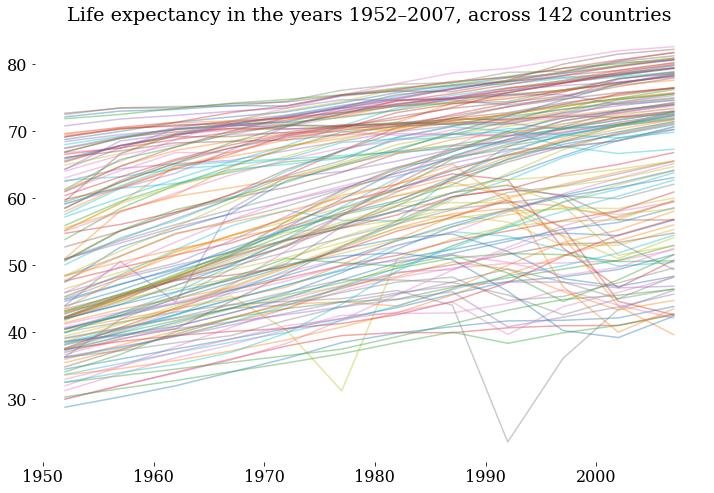
\includegraphics{figures/engcomp2lesson4-life-expectancy.png}
\caption{From: \url{http://go.gwu.edu/engcomp2lesson4}}
\end{figure}

Jupyter notebooks are essential tools of connection -- tools that engage
learners in transitions in their thinking. The opportunity of
intermingling computation into a narrative, creating a conversation with
data is a powerful and effective form of communication. With Jupyter,
you now have a new form of content to create and share with learners:
\emph{computable content}. In a world where every subject matter can
have a data-supported treatment, where computational devices are
omnipresent and pervasive, the union of natural language and computation
creates compelling communication and learning opportunities.

\subsection{2) Participation}\label{participation}

Engaging students in your courses requires their participation and
interaction with you, their peers, and/or the content {[}Michael Moore,
1989{]}. How, when, and why you use student participation in yours will,
of course, depend on your goals, the specific objectives for teaching
the content within your course, your students, and other factors. Using
notebooks, however, encourages participation and gives you more tools
for promoting participation. Notebooks can connect students to authentic
external audiences as well. Students can, for example, consume notebooks
from other classes, and publish notebooks where others can read them.

\subsubsection{Real World Experience -- bringing concepts to
life}\label{real-world-experience-bringing-concepts-to-life}

Notebooks are living documents, meaning they can be edited to respond to
questions or input from students and used a conversation piece during a
lecture or presentation.

\begin{verbatim}
_Our group uses Jupyter notebooks as "apps" to demonstrate concepts in geophysics. These notebook-apps connect numerical simulations to widgets and relevant plots. In the classroom, we ask students to help define input parameters based on an application or case study that they are interested in. Prior to displaying the results, we ask students to build a mental image of their expectations. If the resultant image matches their expectations, then we have reinforced a concept, and if not, it is an opportunity to learn. We as instructors can interactively engage with students' questions by updating the inputs to the simulation in order to explore concepts with them. Students have access to the same notebooks through free web-platforms like Binder, so simply by following a link, they can take the steering wheel and engage with the concepts on their own. Notebooks bring the concepts to life and serve as a conversation piece for the interaction between learners and educators. -- Lindsey Heagy_
\end{verbatim}

\begin{figure}
\centering
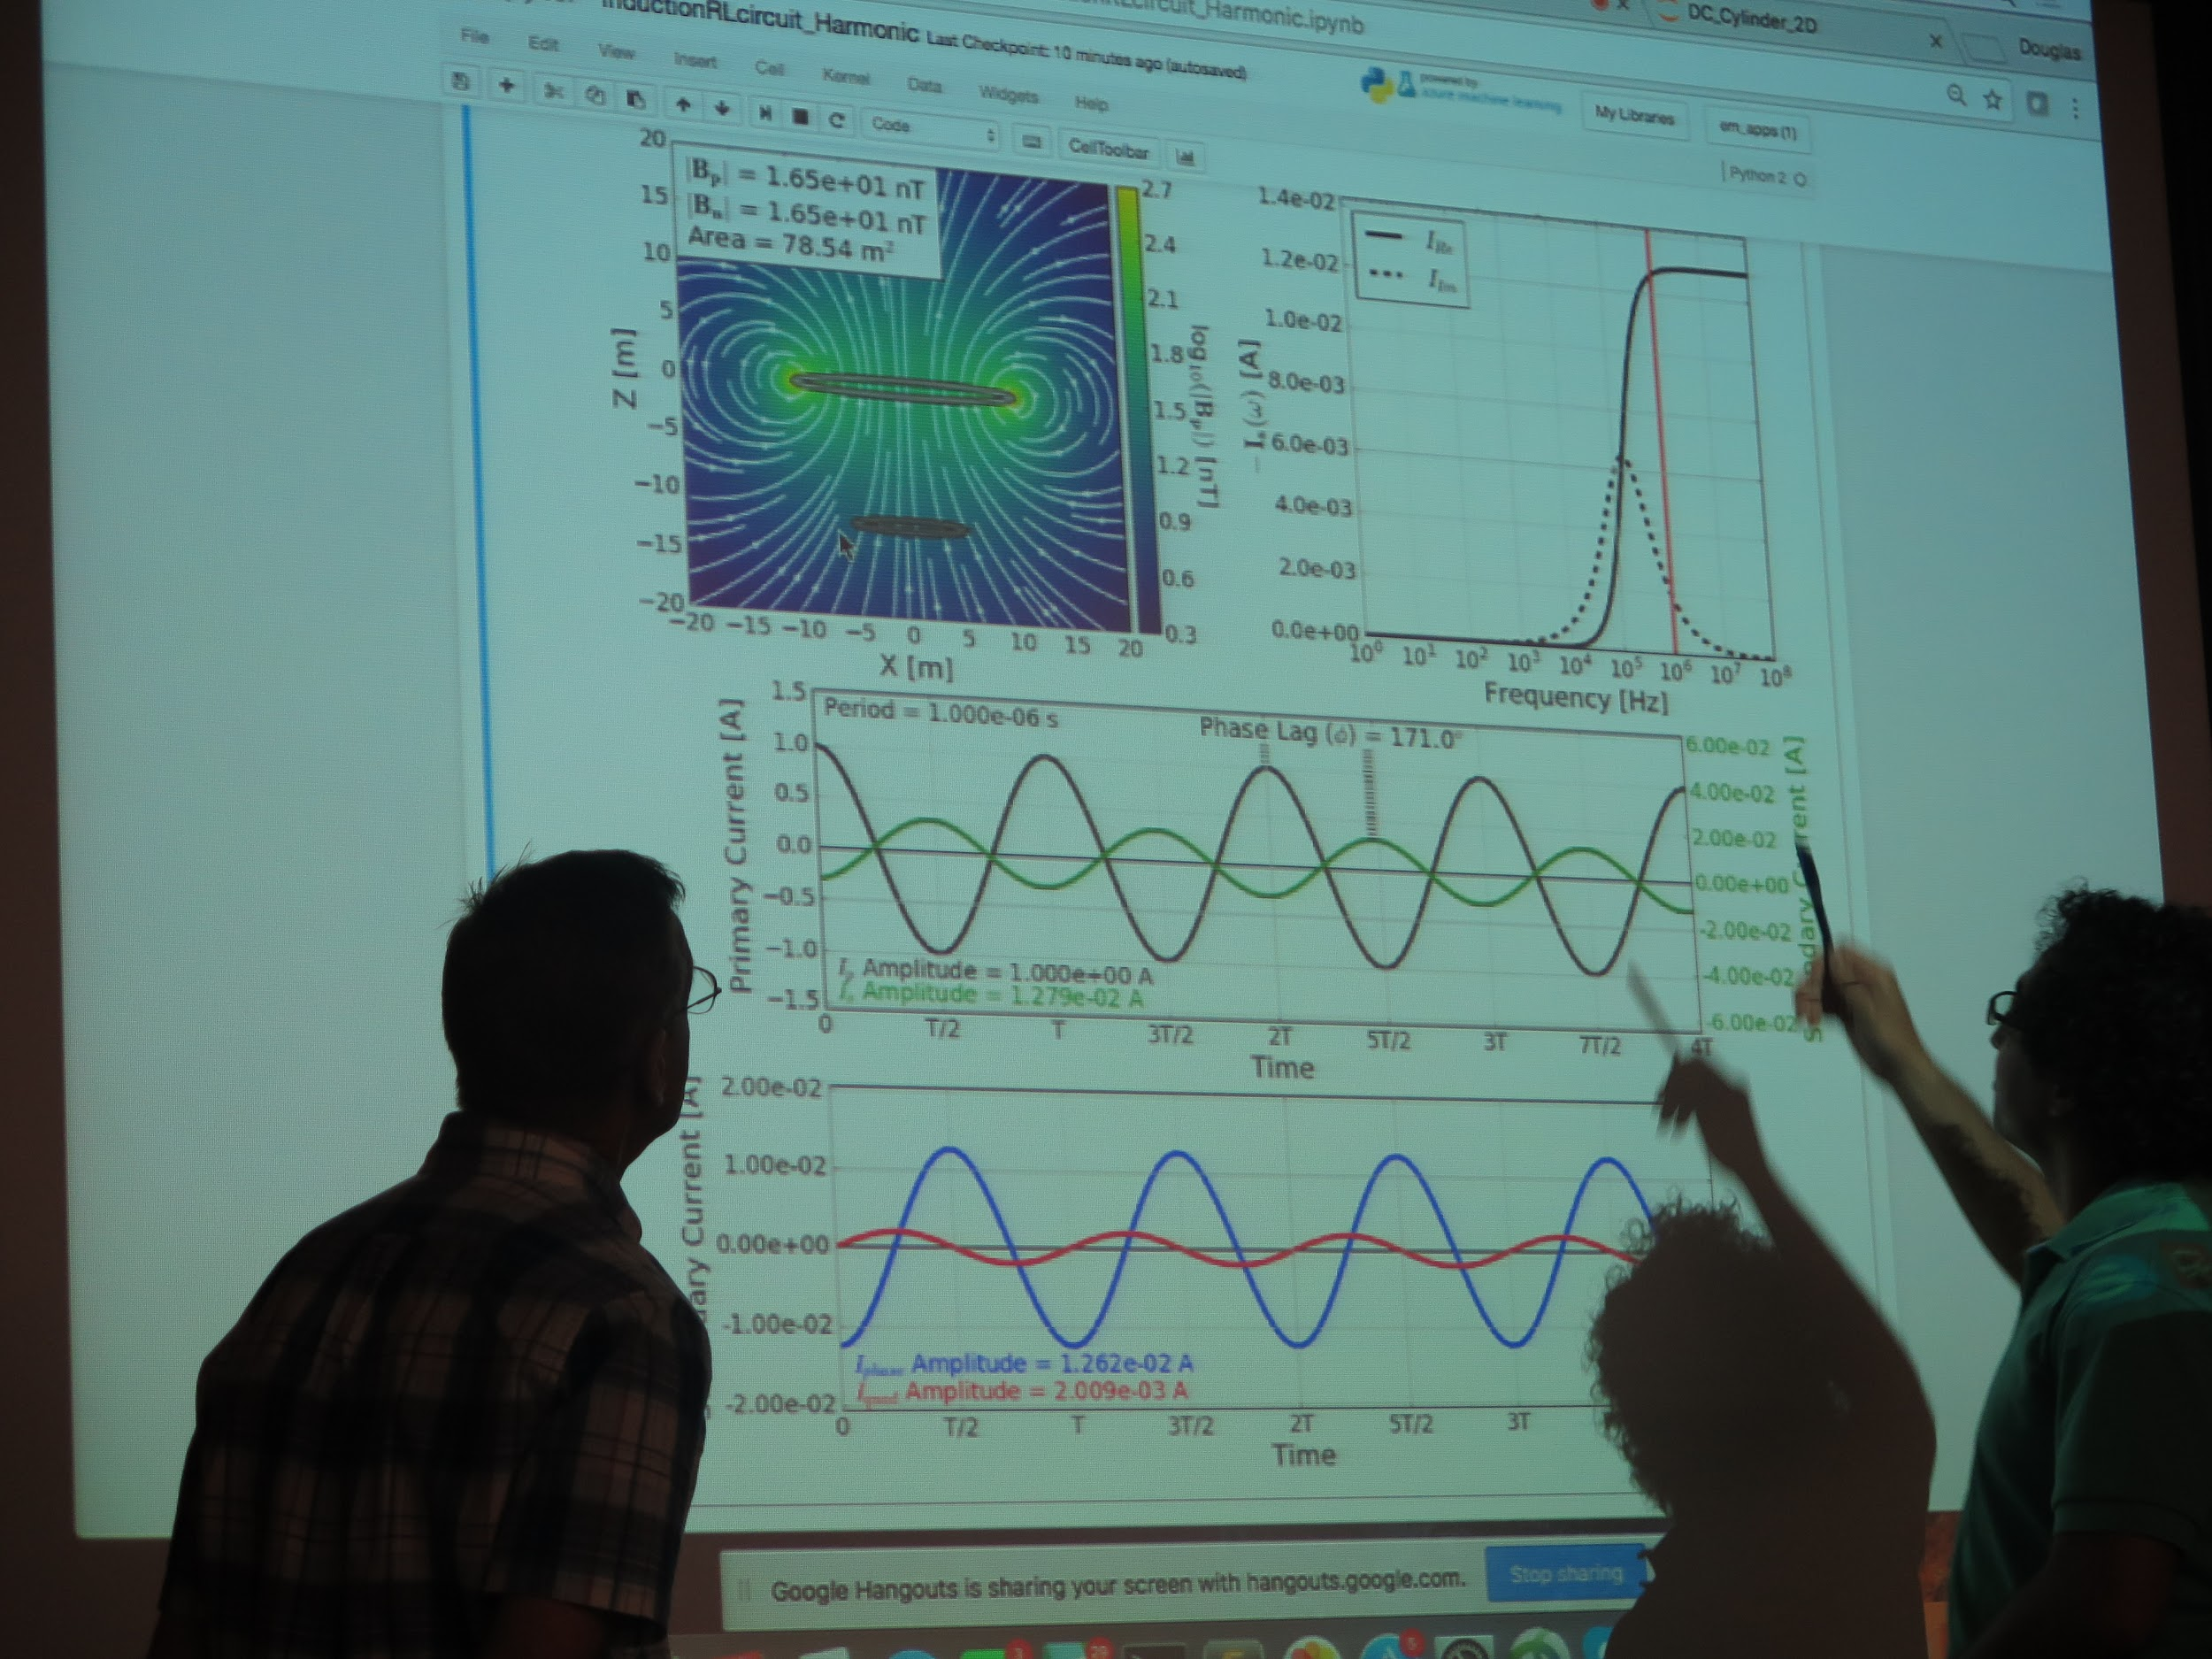
\includegraphics{figures/oldenburg-geosci.jpg}
\caption{Dr.~Douglas Oldenburg (left) engaging with a student during a
short course on geophysical electromagnetics (\url{https://geosci.xyz}).
Photo credit: Seogi Kang}
\end{figure}

\subsubsection{Real World Experience -- Ticket to
leave}\label{real-world-experience-ticket-to-leave}

Another example of generating participation in the classroom with
Jupyter notebooks is the Activity magic, available as an extension. It
creates what has been called a ``ticket to leave'' (or ``exit ticket'')
via the notebook. The idea of a ``ticket to leave'' is an excellent way
to end a class or lab. Briefly, it is just a survey that you give the
students (see figure). Often, these surveys are given via a Personal
Response System (also known as ``clickers'' or PRS) or cell phones.
There are a few uses of such surveys:

\begin{enumerate}
\def\labelenumi{\arabic{enumi}.}
\tightlist
\item
  Give the instructor some feedback on the students' understanding, as a
  whole
\item
  Provide time and opportunity for students to review and synthesize
  today's materials
\item
  Allow the students to apply their recent knowledge to a novel problem
\item
  An additional instance to learn the materials
\end{enumerate}

\begin{figure}
\centering
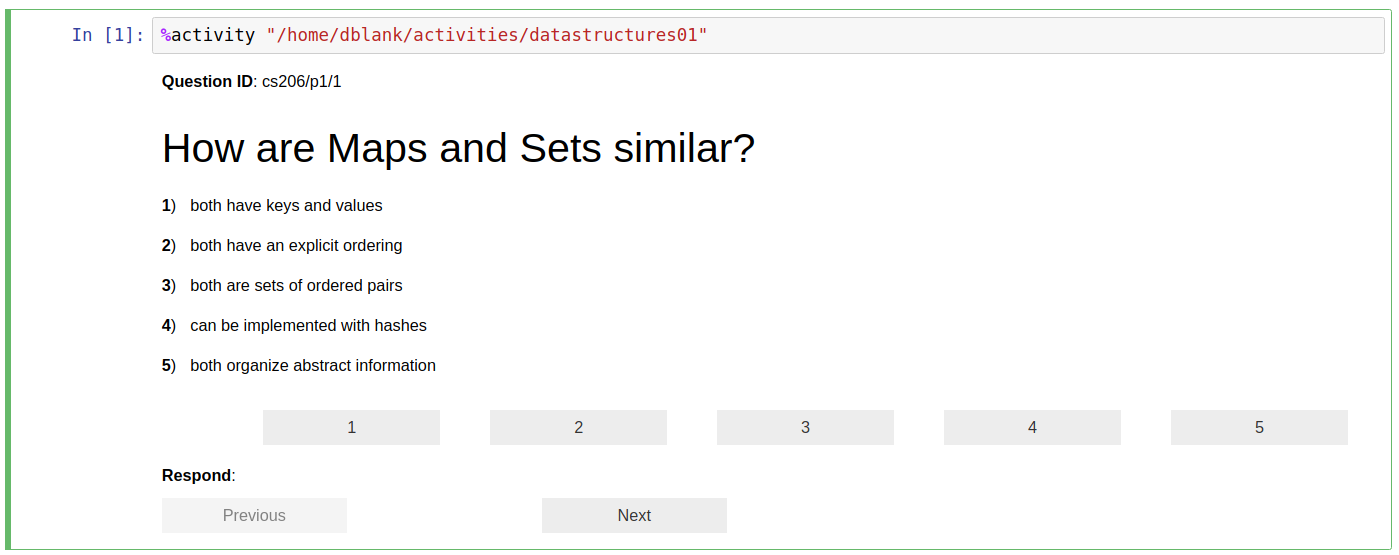
\includegraphics{figures/activity-magic-student.png}
\caption{Example of the Activity magic seen from the students view. A
question, with multiple choice answers is shown, with buttons for their
input.}
\end{figure}

These questions do not typically require much time to answer, but are
meant to capture the essence of the conversation of the class. After a
minute or so to contemplate the question, the students select their
answer (by clicking one of the buttons), and instructor shows the
gestalt results (see figure).

\begin{figure}
\centering
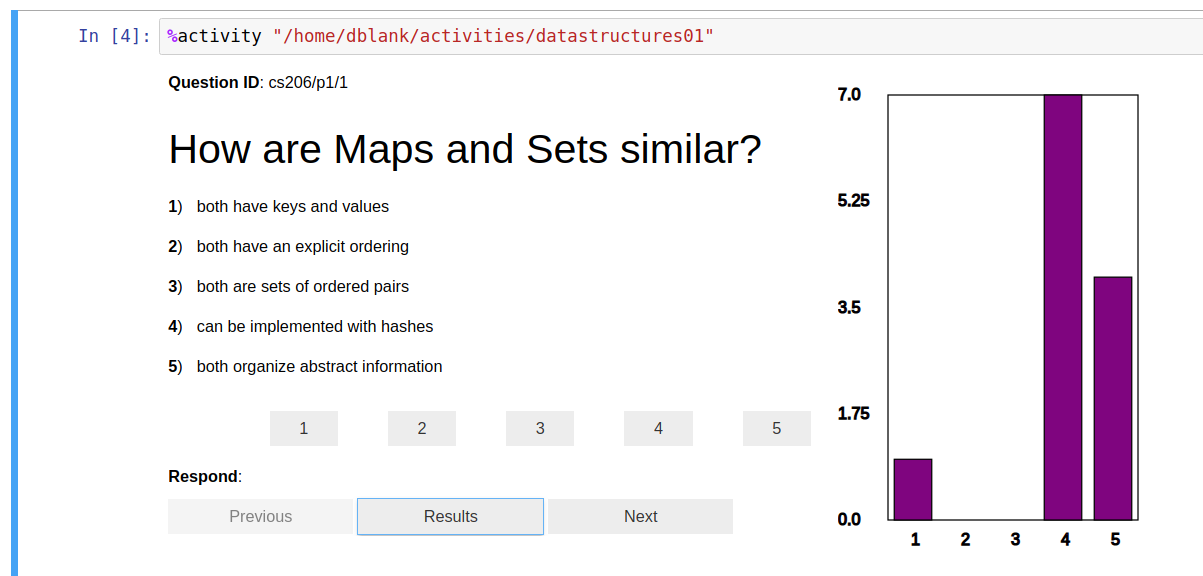
\includegraphics{figures/activity-magic-instructor.png}
\caption{The Activity magic, from the the instructor's perspective. The
barchart is shown on the project once all of the students have had a
chance to respond.}
\end{figure}

Good ``exit ticket'' questions can be domain specific questions, but can
also be metacognitive questions (about one's learning style, for
example), or high-level organizational questions (e.g., ``what was the
goal of today's discussion?''). We recommend leaving enough time at the
end of class (perhaps 10 minutes) to have a full and complete wrap-up
discussion. After the discussion, you may wish to adjust the following
class meeting if you feel that not enough students had the insight you
were aiming for. For more information on ``tickets to leave'' see
\url{https://www.brown.edu/sheridan/teaching-learning-resources/teaching-resources/course-design/classroom-assessment/entrance-and-exit/sample}

\subsection{3) Increasing Understanding}\label{increasing-understanding}

Within any course you will typically try to achieve a diverse set of
objectives. Benjamin Bloom
(\url{https://en.wikipedia.org/wiki/Bloom\%27s_taxonomy}) provided a
framework for the detailed objectives we want to achieve, ranging from
basic knowledge (such as, terminology, specific facts, trends and
sequences, classifications and categories, etc.) all the way to ability
to evaluate and create (such as, abstract relationships, judgments but
based criteria, original works). Achieving the former (i.e., basic
knowledge and comprehension) is far easier to achieve that understanding
(i.e., evaluation and creation); yet, most often we, as educators, are
striving for increasing the complex understanding of our students on the
topics we are teaching. The good news is that notebooks offer a valuable
tool for teaching toward understanding -- moving students, for example,
from passively viewing course content to exploring, analyzing,
synthesizing, and evaluating the content in active ways.

\subsubsection{Real World Experience -- Guiding Learners at their Own
Pace}\label{real-world-experience-guiding-learners-at-their-own-pace}

The fundamental theory behind Computational Fluid Dynamics (CFD) used in
Aerospace Engineering is based on understanding the Navier-Stokes
equations. ``CFD Python'' is a collection of Jupyter Notebooks based on
a practical module that I began using in class in my Computational Fluid
Dynamics (CFD) course at Boston University in 2009. The 5-week module
develops worked examples that build on each other to incrementally guide
the learner to create a program to solve the Navier-Stokes equations of
fluid mechanics, in 12 steps.

\begin{verbatim}
_In 2013, I was invited to teach a 2 day mini-course in the Latin-American School in High-Performance Computing, in Argentina. The Jupyter Notebooks platform allowed me to create a guided narrative to support learners with different background experience and knowledge. For that event, we wrote Notebooks based on the CFD course module, to use as instructional scaffolding in the minicourse. Twenty students worked through the notebooks as self-paced lessons, while I went from desk to desk asking and answering questions. About four of the students completed all 12 steps in the 2 days, a bulk of them achieved up to about Step 8, and a few of them lagged behind in Steps 4 or 5 by the end of the course. For those who completed the full module, they had achieved in 2 days what my regular students in the classroom normally took 5 weeks to do. Seeing that was an eye-opening moment: both the power of worked examples in code, and the ability to allow learners to follow their own pace made a remarkable difference in these learners. -- Lorena Barba_
\end{verbatim}

Based on the experience developing the ``CFD Python'' learning module
{[}\emph{Barba et. Al 2018 }\url{https://doi.org/10.21105/jose.0002}{]},
this basic design pattern was adopted for creating lessons using
computable content:

\begin{enumerate}
\def\labelenumi{\arabic{enumi}.}
\tightlist
\item
  Break it down into small steps
\item
  Chunk small steps into bigger steps
\item
  Add narrative and connect
\item
  Link out to documentation
\item
  Interleave easy exercises
\item
  Spice with challenge questions/tasks
\item
  Publish openly online
\end{enumerate}

This was particularly helpful for student understanding.

\subsection{4) Increasing Student's
Performance}\label{increasing-students-performance}

The goal of learning is often actualized through the performance of
students. This is routinely most visible by what we attempt to assess
during and at the end of instruction. Using notebooks we can create a
variety of a performance opportunities for students, thereby giving them
more opportunities for practice and feedback, as well as more
opportunities for us, as instructors, to assessment their ability to
perform.

\subsubsection{Real World Experience -- The Worked-example
effect}\label{real-world-experience-the-worked-example-effect}

The worked-example effect is the best known and most widely studied of
the cognitive load effects {[}Sweller, J. (2006){]}. It refers to
providing full guidance on how to solve a problem, resulting in better
student performance than problem-solving conditions with no guidance.
For complex tasks, inexperienced or beginner learners benefit the most
from the worked-examples procedure. One study (Chen et al., 2015)
concludes that: ``worked example effect occurs for complex, high-element
interactivity materials that impose a heavy working memory load'' and
``when dealing with complex material that learners may have difficulty
understanding, high levels of guidance are likely to result in enhanced
performance over lower levels of guidance.'' This research-based
guidance seems especially relevant for teaching novice programmers to
use computation in the context of their subject matter (science,
engineering, or other).

\subsection{5) Increasing Students' Preparation for Their
Career}\label{increasing-students-preparation-for-their-career}

In preparing students to apply what they have learned, striving to align
what happens in the course with what they will experience in their
career is important. From using parallel software to mirroring
workflows, we want our students to experience and be prepared for the
workplace. Recognizing, of course, that workplaces are not static and
the skills required for a career are always emerging, using notebooks
provides a flexible platform to build skills and build portfolios of
what students can do.

\subsubsection{Real World Experience -- Publishing a data narrative as a
demonstration of industry
ability}\label{real-world-experience-publishing-a-data-narrative-as-a-demonstration-of-industry-ability}

For Data Science careers, a publicly shared narrative about a data
analytics project goes a long way at demonstrating the student's
potential at an interview. Elizabeth Wicks has her students develop a
Jupyter notebook that tells the story of a data munging and analysis
project done in the class. The students then publish this notebook to
their Github profile pages. Being that Jupyter is one of the most
popular ways in industry to communicate data science results, the
students have a very valuable key to a potential career.

TODO: Add quote from Elizabeth

\section{Student benefits}\label{student-benefits}

Creating opportunities for students to develop as learners stretch
beyond the boundaries of any specific course where you may use
notebooks. By enriching their learning experience in your course, you
will help them develop valuable skill-sets and mind-sets that they will
take with them into other courses and into their career.

\subsubsection{Computational Thinking}\label{computational-thinking}

Jupyter Notebooks support a wide range of learning goals. Its
interactivity enables building intuitive understanding of domain
knowledge, such as the understanding of a mechanical response of a
system while varying parameters or understanding how an algorithm
behaves. Notebooks can also help teach effective communication skills,
combining prose with graphics into a strong narrative. Finally,
notebooks can support teaching or strengthening programming skills, by
combining code with text descriptions and visualizations. Even if a
notebook is designed to be consumed passively, the exposure to code
helps show students how to do something---and that they can do it
themselves. This also helps demystify coding for students who do not
view themselves as traditional ``computer science'' types.

Using notebooks, you can create rich learning experiences that link
together the core foundations of computational thinking:

\begin{itemize}
\tightlist
\item
  \emph{Decomposition}: Breaking down data, processes, or problems into
  smaller, manageable parts
\item
  \emph{Pattern Recognition}: Observing patterns, trends, and
  regularities in data
\item
  \emph{Abstraction}: Identifying the general principles that generate
  these patterns
\item
  \emph{Algorithm Design}: Developing the step by step instructions for
  solving this and similar problems (see
  \url{https://usr55.dayforcehcm.com/CandidatePortal/en-US/myeyedr/Posting/View/8612?fbclid=IwAR0BVRfn38L7PMftCSbYY_n7IZDhMba0HA7Mmn78ASu5rRIivvPtcAYqxWs})
\end{itemize}

\subsubsection{Open-source}\label{open-source}

Integrating notebooks into classes also exposes students to a large and
growing ecosystem of open-source tools. This supports their education,
but also provides experience in the same environment of tools used in
industries in high demand for trained employees, such as data science
and machine learning. The open-source nature of these tools also ensures
that course content remains accessible and affordable to all
students---including those outside the traditional university
environment.

Unlike proprietary notebook technologies such as Mathematica, or
specific programming languages/environments such as Matlab or C++, the
barriers to entry for students learning with Jupyter notebooks can be
extremely low. At a minimum, during a lecture, students can simply
watch/read an interactive demo using a notebook, to replace slides or
lecture notes. On their own, using a cloud service such as Binder or
JupyterHub, students can open any modern web browser to some address and
interact with a notebook (an example of this technology can be found at
\url{https://jupyter.org/try}) , without needing any installation or
configuration. In the most complicated case, students can install
Anaconda and follow simple instructions to install the Jupyter Notebook,
which works and looks the same on all platforms---and is free and open
source.

\subsubsection{Active learning}\label{active-learning}

Thanks to their interactivity, notebooks enable a spectrum of active
learning methods, which have been shown to increase performance in
science, engineering, and mathematics {[}Freeman et al. 2018{]}. To
start, students can consume notebook content by reading and running
notebooks, then move to editing or completing notebooks as assignments.
This allows students to focus on the content and concepts, rather than
just note-taking.

At the top of Bloom's Taxonomy is pure creation, where students can, for
example, author complete computational essays. In both cases, notebooks
support courses where students have a wide range of experience and
ability: students who need help can rely on the scaffolding of prose
explanations and existing code, while also providing room to stretch and
explore for more-experienced students. The additional annotation and
prose that accompanies code also helps support non-traditional learners
and students from underrepresented groups who may have less initial
experience/comfort with programming.

Instilling the habits of active learning, through the use of notebooks,
will also provide benefits beyond the boundaries of your course.
Interactivity drives engagement, interest, and exploration of concepts.
Engaged students in your course, are more likely to be engaged learner
in other courses and beyond.

\section{Instructor benefits}\label{instructor-benefits}

Notebooks can be adopted at a variety of levels and formats, offering
flexibility based on the needs of a course and comfort/interest level of
the instructor: in-class demos, interactive labs, auxiliary material
(e.g., book replacements, lecture note supplements), assignments, or
full course content in a flipped learning environment. Notebooks offer a
route to active learning methods for instructors without experience of
them, but do not force a particular teaching style.

At a minimum, notebooks can be used to make publishable and interactive
lecture notes that blend narrative text, images, videos with image and
results to present the concepts. Furthermore, these course materials can
be developed gradually, starting with a low-effort draft to a
more-polished, publishable document that can be easily extended over
time---and adopted by others. The growth of open-source communities
around software tools and educational resources creates more
opportunities for the re-use and adaptation of existing resources.

While many notebook authors do use Python, the Jupyter Notebook supports
many languages, so students (and instructors) are not tied to one
specific language. Indeed, the name Jupyter comes from three languages:
Julia, Python, and R. Furthermore, these (free) tools have minimal
barriers to entry---using a cloud infrastructure means students and
instructors do not have to install anything, while in the ``worst'' case
installations require a few command-line excursions, but these are free,
openly available, and cross-platform.

\section{Conclusions}\label{conclusions}

We hope that this chapter has illustrated that teaching with Jupyter
notebooks can be valuable for you and your student. We have notebooks to
be a tool that can increase student engagement, participation,
understanding, performance, and preparation for their careers. These are
substantial accomplished that can be achieved in a variety of
disciplines and content areas. Using several real world examples, we
attempted to illustrate the numerous ways teachers are using notebooks.
Hopefully these, when combined with the chapters that follow, will guide
you in 1) supporting your students' learning, 2) giving you confidence
that you can use notebooks, 3) help you understand the necessary
logistics, and 4) help give you clear expectations of what can be
accomplished with Jupyter notebooks.

\chapter{About the Authors}\label{authors}

\section{Project Lead}\label{project-lead}

\subsection{Lorena A. Barba}\label{lorena-a.-barba}

\begin{itemize}
\tightlist
\item
  George Washington University
\item
  \href{mailto:labarba@email.gwu.edu}{\nolinkurl{labarba@email.gwu.edu}}
\item
  \href{https://twitter.com/LorenaABarba}{@LorenaABarba}
\end{itemize}

Lorena A. Barba is Associate Professor of Mechanical and Aerospace
Engineering at the George Washington University. She adopted Jupyter in
2013 and since then used it in every course she teaches. Her open course
materials are well known and used by thousands of learners:
\href{http://lorenabarba.com/blog/cfd-python-12-steps-to-navier-stokes/}{CFD
Python} and
\href{https://github.com/numerical-mooc/numerical-mooc}{Numerical MOOC}
are the best examples.

\section{Authors at the sprint}\label{authors-at-the-sprint}

\subsection{Lecia J. Barker}\label{lecia-j.-barker}

\begin{itemize}
\tightlist
\item
  University of Colorado Boulder
\item
  \href{mailto:lecia.barker@colorado.edu}{\nolinkurl{lecia.barker@colorado.edu}}
\item
  \href{https://twitter.com/leciab}{@leciab}
\end{itemize}

\href{https://www.colorado.edu/cmci/people/information-science/lecia-barker}{Lecia
Barker} is an Associate Professor and Associate Chair of Undergraduate
Studies in the
\href{https://www.colorado.edu/cmci/infoscience}{Department of
Information Science} at the University of Colorado Boulder. She is also
a Senior Research Scientist for the
\href{https://www.ncwit.org/}{National Center for Women \& IT}. Her
research group is studying the
\href{https://csteachingpractices.wordpress.com/}{diffusion and adoption
of teaching practices} in undergraduate computer science. Lecia holds a
Ph.D.~in Communication from CU Boulder and an MBA in Marketing from San
Diego State University.

\subsection{Douglas Blank}\label{douglas-blank}

\begin{itemize}
\tightlist
\item
  Bryn Mawr College
\item
  \href{mailto:dblank@brynmawr.edu}{\nolinkurl{dblank@brynmawr.edu}}
\item
  \href{https://twitter.com/dougblank}{@dougblank}
\end{itemize}

\href{https://cs.brynmawr.edu/~dblank/}{Douglas Blank} is Associate
Professor in the \href{https://cs.brynmawr.edu/}{Department of Computer
Science} at \href{http://brynmawr.edu/}{Bryn Mawr College}, a small,
all-women's college outside of Philadelphia, PA, USA. He has a joint
Ph.D.~in Cognitive Science and Computer Science from Indiana University,
Bloomington. For over 20 years, Douglas has taught all levels of
Computer Science. For the last 4 years, he has used Jupyter notebooks
exclusively in the classroom. Douglas has published in the areas of
Computer Science Education, Robotics, Artificial Intelligence, and Deep
Learning. He is on the advisory board of
\href{https://www.engage-csedu.org}{Engage-CSEdu.org}, a joint project
between Google and the National Center for Women and Information
Technology (NCWIT). Douglas also writes text and code at his website
\href{http://douglasblank.com}{douglasblank.com}.

\subsection{Jed Brown}\label{jed-brown}

\begin{itemize}
\tightlist
\item
  University of Colorado Boulder
\item
  \href{mailto:jed@jedbrown.org}{\nolinkurl{jed@jedbrown.org}}
\item
  \href{https://twitter.com/five9a2}{@five9a2}
\end{itemize}

\href{https://jedbrown.org/}{Jed Brown} is an Assistant Professor of
Computer Science at the University of Colorado Boulder. He has been
teaching numerical and scientific computing courses using Jupyter
Notebook and nbgrader for three years, and leads a research group that
develops computational methods and community software for computational
science.

\subsection{Allen Downey}\label{allen-downey}

\begin{itemize}
\tightlist
\item
  Olin College
\item
  \href{mailto:downey@allendowney.com}{\nolinkurl{downey@allendowney.com}}
\item
  \href{https://twitter.com/AllenDowney}{@AllenDowney}
\end{itemize}

\href{http://www.allendowney.com/wp/}{Allen Downey} is a professor of
Computer Science at Olin College and the author of a series of
open-source textbooks related to software and data science, including
\emph{Think Python}, \emph{Think Bayes}, and \emph{Think Complexity},
published by O'Reilly Media. These books, and the classes based on them,
use Jupyter notebooks extensively. Prof Downey holds a Ph.D.~in computer
science from U.C. Berkeley, and M.S. and B.S. degrees from MIT.

\subsection{Tim George}\label{tim-george}

\begin{itemize}
\tightlist
\item
  Project Jupyter
\item
  \href{mailto:tgeorgeux@gmail.com}{\nolinkurl{tgeorgeux@gmail.com}}
\end{itemize}

\href{https://www.tgeorgeux.com/}{Timothy George} is the Lead UI/UX
Designer for \href{https://jupyter.org/}{Project Jupyter}, focusing
primarily on JupyterLab. In addition to his formal duties, Tim is also
in working with Jupyter on design strategy, future products, governance,
diversity and inclusion. He studied HCI at UC Irvine's Donald Bren
School of Informatics and Computer Science where he received a Master's
Degree.

\subsection{Lindsey Heagy}\label{lindsey-heagy}

\begin{itemize}
\tightlist
\item
  University of California Berkeley
\item
  \href{mailto:lindseyheagy@gmail.com}{\nolinkurl{lindseyheagy@gmail.com}}
\item
  \href{https://twitter.com/lindsey_jh}{@lindsey\_jh}
\end{itemize}

\href{https://www.lindseyjh.ca/}{Lindsey Heagy} is a Postdoctoral
Researcher at the University of California Berkeley working on Project
Jupyter and Jupyter in the geosciences. She recently completed her PhD
at the University of British Columbia in geophysics. She is a project
leader of \href{http://geosci.xyz}{GeoSci.xyz}, an effort to build
collaborative, interactive, web-based textbooks in the geosciences, and
a core contributor to \href{https://www.simpeg.xyz/}{SimPEG}, an open
source framework for geophysical simulation and inversions. The
GeoSci.xyz project relies heavily on Jupyter for making the content come
to life.

\subsection{Kyle Mandli}\label{kyle-mandli}

\begin{itemize}
\tightlist
\item
  Columbia University
\item
  \href{mailto:kyle.mandli@columbia.edu}{\nolinkurl{kyle.mandli@columbia.edu}}
\item
  \href{https://twitter.com/KyleMandli}{@KyleMandli}
\end{itemize}

\href{https://www.columbia.edu/~ktm2132}{Kyle Mandli} is an Assistant
Professor in the Department of Applied Physics and Applied Mathematics
at Columbia University. He has developed a set of openly available
course notes centered around Jupyter notebooks and uses Jupyter for
homework in conjunction with nbgrader. His other research interests
include development of computational methods for coastal hazards such as
storm surge and tsunamis.

\subsection{Jason K. Moore}\label{jason-k.-moore}

\begin{itemize}
\tightlist
\item
  University of California, Davis
\item
  \href{mailto:jkm@ucdavis.edu}{\nolinkurl{jkm@ucdavis.edu}}
\item
  \href{https://twitter.com/moorepants}{@moorepants}
\end{itemize}

\href{http://moorepants.info/}{Jason K. Moore} is an Assistant Teaching
Professor of Mechanical and Aerospace Engineering at the University of
California, Davis. He currently teaches dynamics and mechanical design
related courses. He utilizes Jupyter notebooks to teach modeling and
simulation and is working on a
\href{https://moorepants.github.io/resonance}{textbook about Mechanical
Vibrations}. He is responsible for the Jupyter related features in the
\href{http://libretexts.org}{LibreTexts project} and is also a core
developer of the \href{http://sympy.org/}{SymPy} and
\href{http://pydy.org/}{PyDy} projects which utilizes Jupyter for
training workshops, e.g.
\href{https://www.sympy.org/scipy-2017-codegen-tutorial/}{PyDy Tutorial}
and \href{https://github.com/pydy/pydy-tutorial-human-standing}{SymPy
Code Generation Tutorial}. Jason has PhD, MSc, and BSc degrees in
mechanical engineering from UC Davis and Old Dominion University.

\subsection{David Lippert}\label{david-lippert}

\begin{itemize}
\tightlist
\item
  Leidos
\end{itemize}

David Lippert is a software engineer at
\href{https://www.leidos.com}{Leidos} in Arlington, Virginia. He
utilizes Jupyter notebooks primarily for exploratory data analysis and
for training and evaluating machine learning algorithms. He has written
Jupyter notebooks to create new Dr.~Seuss sonnets and to evaluate if the
\href{https://www.rottentomatoes.com/about}{Rotten Tomatoes Tomatometer}
can be trusted. He has a BA in computer science from Middlebury College.

\subsection{Kyle Niemeyer}\label{kyle-niemeyer}

\begin{itemize}
\tightlist
\item
  Oregon State University
\item
  \href{mailto:kyle.niemeyer@oregonstate.edu}{\nolinkurl{kyle.niemeyer@oregonstate.edu}}
\item
  \href{https://twitter.com/kyleniemeyer}{@kyleniemeyer}
\end{itemize}

\href{https://niemeyer-research-group.github.io/}{Kyle Niemeyer} is an
Assistant Professor of Mechanical Engineering in the School of
Mechanical, Industrial, and Manufacturing Engineering at Oregon State
University. He teaches courses in numerical and analytical methods for
solving differential equations as well as gas dynamics, and recently
developed a
\href{https://softwaredevengresearch.github.io/syllabus/}{graduate
course on software development for engineering research}. His research
group develops and applies methods for modeling combustion and
chemically reacting fluid flows. He is also on the steering committee of
the \href{https://cantera.org/}{Cantera} open-source project for
chemical kinetics, thermodynamics, and transport processes.

\subsection{Ryan Watkins}\label{ryan-watkins}

\begin{itemize}
\tightlist
\item
  George Washington University
\item
  \href{mailto:rwatkins@gwu.edu}{\nolinkurl{rwatkins@gwu.edu}}
\item
  \href{https://twitter.com/parsingscience}{@parsingscience}
\end{itemize}

\href{https://gsehd.gwu.edu/directory/ryan-watkins}{Ryan Watkins} is a
Professor of Educational Technology at George Washington University in
Washington DC. He leads the
\href{https://go.gwu.edu/phd}{Human-Technology Collaboration (HTC)} PhD
program area, and he teaches courses in needs assessment, instructional
design, and research methods. Ryan's research focuses on how people and
organizations define and assess needs. He is co-host of
\href{https://parsingscience.org/}{Parsing Science}, a podcast where
researchers share the stories behind their science. He also developed
the \href{https://wesharescience.org/}{We Share Science} platform for
sharing video abstracts of research.

\subsection{Richard West}\label{richard-west}

\begin{itemize}
\tightlist
\item
  Northeastern University
\item
  \href{mailto:R.West@northeastern.edu}{\nolinkurl{R.West@northeastern.edu}}
\item
  \href{https://twitter.com/richardhwest}{@richardhwest}
\end{itemize}

\href{https://web.northeastern.edu/comocheng/}{Richard West} is
Associate Professor of Chemical Engineering at Northeastern University
in Boston. He leads a research group in computational modeling for
complex reacting systems like combustion or catalysis. He is a core
member of the \href{https://cantera.org/}{Cantera} open-source project.
As well as in an elective on ``computational modeling in chemical
engineering'', he has integrated Python and Jupyter into core classes on
chemical kinetics and reactor design, at both the undergraduate and
graduate levels. As part of his NSF CAREER award, he is developing
modules to teach students to use Python and SciPy to solve chemical
engineering problems.

\subsection{Elizabeth Wickes}\label{elizabeth-wickes}

\begin{itemize}
\tightlist
\item
  University of Illinois at Urbana-Champaign
\item
  \href{mailto:wickes1@illinois.edu}{\nolinkurl{wickes1@illinois.edu}}
\item
  \href{https://twitter.com/elliewix}{@elliewix}
\end{itemize}

\href{https://ischool.illinois.edu/people/elizabeth-wickes}{Elizabeth
Wickes} is a Lecturer at the School of Information Sciences at the
University of Illinois at Urbana-Champaign. She teaches foundational
programming from an information and data sciences perspective, as well
as other coursework on open data and reproducibility. Her programming
course lectures are written in Jupyter Notebooks and the class is taught
via live coding.

\subsection{Carol Willing}\label{carol-willing}

\begin{itemize}
\tightlist
\item
  Cal Poly San Luis Obispo
\item
  \href{mailto:willingc@gmail.com}{\nolinkurl{willingc@gmail.com}}
\item
  \href{https://twitter.com/WillingCarol}{@WillingCarol}
\end{itemize}

\href{https://www.willingconsulting.com/about/}{Carol Willing} is a
Research Software Engineer at Cal Poly San Luis Obispo working full-time
on \href{https://jupyter.org/}{Project Jupyter}. She is a Python
Software Foundation Fellow and former Director; a Project Jupyter
Steering Council member; and a core developer on CPython and Jupyter.
Carol has an M.S. in Management from MIT and a B.S.E. in Electrical
Engineering from Duke.

\subsection{Michael Zingale}\label{michael-zingale}

\begin{itemize}
\tightlist
\item
  Stony Brook University
\item
  \href{mailto:Michael.Zingale@stonybrook.edu}{\nolinkurl{Michael.Zingale@stonybrook.edu}}
\item
  \href{https://twitter.com/Michael_Zingale}{@Michael\_Zingale}
\end{itemize}

\href{http://www.astro.sunysb.edu/mzingale/}{Michael Zingale} is an
Associate Professor and computational astrophysicist at Stony Brook
University. He has a PhD from University of Chicago (2000). He
frequently teaches
\href{http://bender.astro.sunysb.edu/classes/numerical_methods/}{numerical
methods} and
\href{http://bender.astro.sunysb.edu/classes/python-science/}{Python for
scientific computing} graduate courses, relying on Jupyter notebooks and
python for much of the presentation. He is an advocate for open
educational resources, as a founder of the
\href{https://github.com/Open-Astrophysics-Bookshelf/}{Open Astrophysics
Bookshelf project} where he hosts his
\href{http://bender.astro.sunysb.edu/hydro_by_example/CompHydroTutorial.pdf}{\emph{Introduction
to Computational Astrophysical Hydrodynamics}} text.

\chapter{Glossary}\label{glossary}

\textbf{Anaconda}: a free, open-source package manager, environment
manager, Python distribution, and collection of
\href{https://docs.anaconda.com/anaconda/packages/pkg-docs/}{over 1,500+
open source packages} including and also Jupyter.
\url{https://www.anaconda.com/what-is-anaconda/}

\textbf{API (Application Programming Interface)}: the exact details of
interacting with software, usually used by other software.

\textbf{Binder}: a hosted service that allows anyone to launch their own
sandboxed notebook environment from a Git repository.
\url{https://mybinder.org}

\textbf{cell}: the area in a Jupyter Notebook where you can enter
markdown, or computer code.

\textbf{cloud, in the}: used to describe software or documents hosted on
a remote computer accessed over the internet.

\textbf{CSV (Comma Separated Values)}: referring to a comma-separated
value file. A plain-text file format such that each line is a list of
data separated by commas.

\textbf{execute}: technical term for having the computer perform the
instructions of your program. Alias for ``run it.''

\textbf{extension, Jupyter}: in this instance, it is not a request for
more time. Rather, a Jupyter extension is a bit of code, often developed
by a third-party, that adds additional functionality to Jupyter. For
example, a popular extension is a Table of Contents creator.

\textbf{flipped classroom}: a teaching style where students work on
their own outside of class to learn new material (sometimes by watching
recorded lectures or reading descriptive/interactive notebooks) and the
come together in the classroom to practice what they've learned through
exercises or experiments.

\textbf{Git}: a popular version control system (VCS) used for keeping
track of changes of files over time.

\textbf{IDE (Integrated Development Environment)}: software that assists
in the development of additional software.

\textbf{Jupyter}: The term ``Jupyter'' may refer to one of a couple of
different things: a community of users and developers focused on the
open source software; the collection of tools and standards that,
together, allow projects like the Jupyter Notebook to operate. The name
refers to the three core programming languages supported: Julia, Python,
and R.

\textbf{JupyterHub}: a cloud service that can provide access to Jupyter
notebooks and environments to multiple users via a modern web browser.
\url{http://jupyter.org/hub}

\textbf{kernel}: In Jupyter, a kernel is the packaging up of a language,
and related programs needed to run it. For example, Python2 and Python3
are separate kernels.

\textbf{LMS (Learning Management System)}: a cloud service that helps
instructors manage aspects of classrooms.

\textbf{load}: how many students can a computer support?

\textbf{Markdown}: a text format that allows for basic formatting
(headers, text styles, links) mixed inline with the text. Markdown files
usually have the extension \texttt{.md} and can be rendered natively by
GitHub and other tools.

\textbf{magic}: a meta-command typically starting with one or two
percent signs. Changes the meaning of the contents of a line (one
percent sign, \texttt{\%}) or the cell (two percent signs,
\texttt{\%\%}) from code to a particular meta-instruction. For example,
\texttt{\%\%R} indicates that the cell contents will be interpreted as
commands to the R language. Magics are kernel-specific (e.g., vary with
the kernel in use).

\textbf{nbgrader}: a tool for creating, handling, and automatically
grading assignments based on Jupyter notebooks.
\url{https://nbgrader.readthedocs.io}

\textbf{nbviewer}: a web application for rendering Jupyter notebooks as
static web pages, providing a URL to share and view them with a modern
web browser. \url{https://nbviewer.jupyter.org}

\textbf{nbconvert}: a tool for converting Jupyter notebooks into other
formats such as PDF, HTML, LaTeX, Markdown, reStructuredText, and
others. \url{https://nbconvert.readthedocs.io}

\textbf{notebook hidden state}: a technical term referring to the value
of variables that may have surprising results due to cells having been
executed in a non-sequential order.

\textbf{open source}: software and documents that are created in a
manner that give you rights to be able to use, and reproduce.

\textbf{pattern}: A ``pattern'' is a technical term referring to an
abstract description of a labeled process. For example, ``wash, rinse,
repeat'' is a common pattern for cleaning various objects.

\textbf{service, JupyterHub}: JupyterHub can take advantage of
additional separate, but integrated, software extensions. These are
called ``services.''

\textbf{script}: a colloquial term for a computer program.

\textbf{unit test}: a technical term for a ``test'' for checking to see
if software is operating correctly.

\textbf{URL (Universal Resource Locator)}: the address of a resource
(e.g., webpage) on the internet.

\textbf{widget}: a user interface (such as buttons, sliders, and
checkboxes) that allow the easy control of hidden computer code.

\bibliography{book.bib,packages.bib}


\end{document}
